\documentclass[spanish, aspectratio=169]{beamer}

\usepackage[es-tabla]{babel}
\usepackage{parskip}
\usepackage[capitalise, noabbrev]{cleveref}
\crefname{table}{\spanishtablename}{\spanishtablename}



\title{
	\textbf{
		Desarrollo de un modelo fundacional estocástico basado en procesos Gaussianos para la clasificación de bioseñales EEG en el diagnóstico asistido del TDAH.
	}
	}
\author{
	Julián David Pastrana Cortés, M.Sc.
	}


\date{}

\begin{document}
	
	
\frame{\titlepage}

\begin{frame}{Motivation}
	\begin{block}{}
		Mental disorders affect cognition, behavior, and emotions of millions of people worldwide. Around 350 million individuals suffer from a mental disorder \emph{Cite this}.
	\end{block}
	
	\begin{columns}[T,onlytextwidth]
		\column{0.33\textwidth}
		\centering
		
\includegraphics[width=0.5\textwidth]{figures/OppositionalDefiantDisorder.png}
		
		\vspace{0.5em}
		\textbf{Oppositional Defiant Disorder}
		
		\column{0.33\textwidth}
		\centering
		
\includegraphics[width=0.5\textwidth]{figures/BipolarDisorder.png}
		
		\vspace{0.5em}
		\textbf{Bipolar Disorder}
		
		\column{0.33\textwidth}
		\centering
		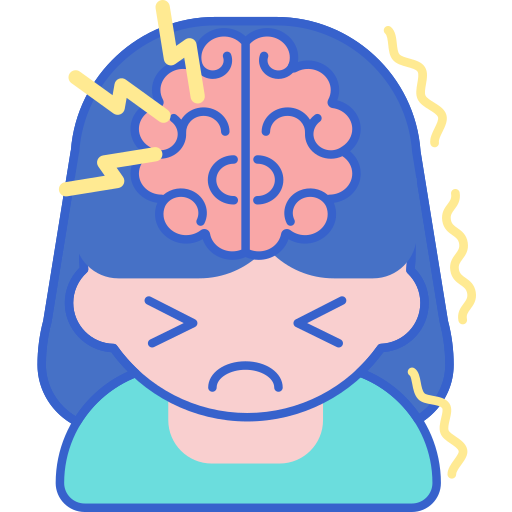
\includegraphics[width=0.5\textwidth]{figures/ADHD.png}
		
		\vspace{0.5em}
		\textbf{Attention Deficit Hyperactivity Disorder}
	\end{columns}
	
	\begin{block}{}
		\textbf{Challenges}: lengthy follow-up, subjective interpretations, inefficient criteria, and limited access to clinical care.
	\end{block}
	
\end{frame}

\begin{frame}{Problem Statement and Research Question}
	
	\begin{table}[htbp]
		\scriptsize
		\begin{tabular}{l >{\centering\arraybackslash}p{1.3cm} >{\centering\arraybackslash}p{1.2cm} >{\centering\arraybackslash}p{1.0cm} >{\centering\arraybackslash}p{1.0cm} >{\centering\arraybackslash}p{1.0cm} >{\centering\arraybackslash}p{1.2cm}}
			\toprule
			\diagbox{\textbf{Model}}{\textbf{Challenge}}          & {Interpretability} & {Nonlinearity} & {Stochasticity} & {Long-term} & {Scalability} & {Output Constraint} \\
			\midrule
			{Physically Driven \cite{Yaseen2018, HKASHANI2016340}} & \textcolor{teal}{\ding{51}} & \textcolor{teal}{\ding{51}} & \textcolor{purple}{\ding{55}} & \textcolor{teal}{\ding{51}} & \textcolor{purple}{\ding{55}} & \textcolor{teal}{\ding{51}} \\ 
			{AR \cite{10.2166/wst.2020.369}}               & \textcolor{teal}{\ding{51}} & \textcolor{purple}{\ding{55}} & \textcolor{teal}{\ding{51}} & \textcolor{teal}{\ding{51}} & \textcolor{teal}{\ding{51}} & \textcolor{purple}{\ding{55}} \\ 
			{NN \cite{w15030505}}               & \textcolor{purple}{\ding{55}} & \textcolor{teal}{\ding{51}} & \textcolor{purple}{\ding{55}} & \textcolor{purple}{\ding{55}} & \textcolor{teal}{\ding{51}} & \textcolor{teal}{\ding{51}} \\ 
			{RNN \cite{doi:10.1080/02626667.2021.1937631}}              & \textcolor{purple}{\ding{55}} & \textcolor{teal}{\ding{51}} & \textcolor{purple}{\ding{55}} & \textcolor{purple}{\ding{55}} & \textcolor{teal}{\ding{51}} & \textcolor{teal}{\ding{51}} \\ 
			{LSTM \cite{8729441, Sahoo2019, 10.1145/3366750.3366756}}             & \textcolor{purple}{\ding{55}} & \textcolor{teal}{\ding{51}} & \textcolor{purple}{\ding{55}} & \textcolor{teal}{\ding{51}} & \textcolor{teal}{\ding{51}} & \textcolor{teal}{\ding{51}} \\ 
			{GP \cite{hensman2014scalable, bruinsma2020scalable}}               & \textcolor{teal}{\ding{51}} & \textcolor{teal}{\ding{51}} & \textcolor{teal}{\ding{51}} & \textcolor{teal}{\ding{51}} & \textcolor{purple}{\ding{55}} & \textcolor{purple}{\ding{55}} \\
			\bottomrule
		\end{tabular}
	\end{table}
	
	
	
	
	
	\begin{block}{Research Question}
		\footnotesize
		How to develop a stochastic foundational model for inference from biological signals that integrates Gaussian processes to support the diagnosis and treatment of mental disorders via EEG signals analysis, considering the variability and inconsistencies present in the datasets?
	\end{block}	
\end{frame}

\begin{frame}{Objectives}
	\vspace{-0.3cm}
	\begin{block}{General Objective}
		\footnotesize
		Develop a learning methodology related to EEG recordings based on a foundational model that integrates labeled and unlabeled databases using self-learning and fine-tuning techniques.
	\end{block}
	
	\vspace{0.4cm}
	\begin{block}{Specific Objectives}
		\footnotesize
		\begin{enumerate}
			\item Develop a foundational model for the classification of biological signals related to EEG recordings, leveraging unlabeled data during the self-learning phase and labeled data for fine-tuning.
			\item Implement a stochastic prediction tool based on Gaussian processes to model uncertainty in the foundational model's predictions.
			\item Design a strategy to manage variability and inconsistency in EEG recording datasets, enabling the effective integration of databases with diverse standards.
		\end{enumerate}
	\end{block}
\end{frame}

	
\end{document}
